\documentclass{article}

\usepackage{graphicx}
\usepackage{lipsum} % for dummy text
\usepackage[shortlabels]{enumitem}

\newenvironment{rulesubsection}[1]{
    \subsection{#1} \label{rule:#1}
    \begin{enumerate}[label=\thesubsection.\arabic{enumi}]
}{
    \end{enumerate}
}

\newcommand{\ruleitem}[1]{\item \label{rule:#1} \textbf{#1.}}

\usepackage{geometry}
 \geometry{
 a4paper,
 total={170mm,257mm},
 left=20mm,
 top=20mm,
}

\usepackage{hyperref}
\hypersetup{
    colorlinks=true,
    linkcolor=blue,
    filecolor=magenta,      
    urlcolor=cyan,
    pdftitle={Overleaf Example},
    pdfpagemode=FullScreen,
}
\newcommand{\ruleref}[1]{\hyperref[rule:#1]{#1}}

\usepackage{background}
\backgroundsetup{contents=
\includegraphics{background.jpg},opacity=0.6,angle=0,scale=0.7}


\begin{document}

\begin{titlepage}
    \begin{center}
        \Huge
        \textbf{Regels van weerwolven}

        \vspace{1cm}
        \textbf{Auteurs} \\
        \vspace{0.5cm}
        \Large
        Alex van Tilburg \\
        Daan van Turnhout \\
        Marijn de Waard \\

        \vfill
        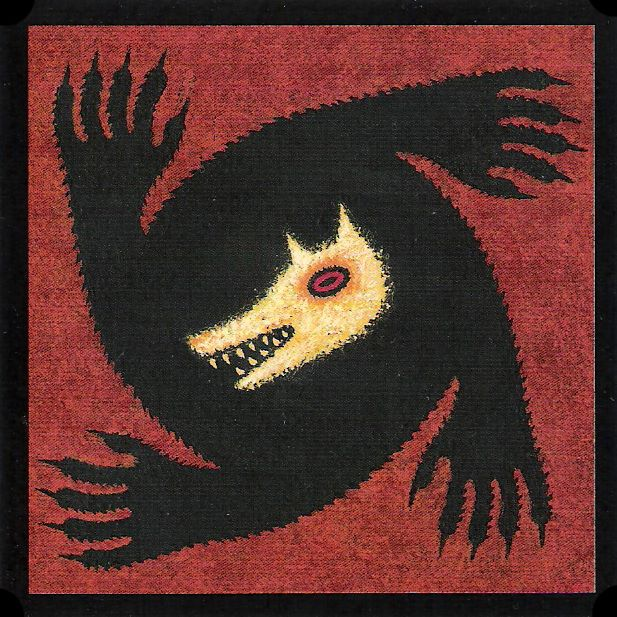
\includegraphics[scale=0.7]{logo.jpg}
        \vfill
    \end{center}
\end{titlepage}

\sffamily

\section*{Introductie}
Dit boek bevat the uitgebereide regels van weerwolven van wakkerdam.
Als je het spel wilt leren, lees dan de algemene spelregels van weerwolven.
Gebruik deze spelregels als je specifieke spelinteracties wilt opzoeken.
\section{Algemene regels}
\begin{rulesubsection}{Tegensprekende regels}
    \ruleitem{Volgorde afhandeling} Als de regels elkaar tegenspreken dan krijgt de regel die hoger staat in het rijtje voorrang:
    \begin{itemize}
        \item wat de \ruleref{Spelleider} zegt
        \item rollen
        \item condities
        \item de rest van de spelregels uit dit boek
        \item de algemene spelregels
    \end{itemize} 
\end{rulesubsection}
\begin{rulesubsection}{Informatie delen}
    \ruleitem{Screenshots} Je mag nooit screenshots delen of berichten van andere mensen doorsturen.
    \ruleitem{Praten} Je mag niet praten tijdens de \ruleref{Nachtfase}, behalve in groepen waar het aangegeven is.
\end{rulesubsection}
\begin{rulesubsection}{Onderhandelingen}
    \ruleitem{Afspraken} Je mag afspraken maken met andere spelers, maar ze zijn nooit bindend.
\end{rulesubsection}
\begin{rulesubsection}{Spel structuur}
    \ruleitem{Fases} Het spel bestaat uit een \ruleref{Dagfase}, \ruleref{Nachtfase}, \ruleref{Zonsopgang} en \ruleref{Zonsondergang}.
    \ruleitem{Dagfase} De Dagfase begint wanneer de \ruleref{Spelleider} de algemene chat open zet. \textit{(Ook al is het 9:00 geweest.)}
    De dagfase eindigt om 20:00. \textit{(Ook al heeft de \ruleref{Spelleider} de algemene chat nog niet gesloten.)}
    \ruleitem{Nachtfase} De nachtfase begint wanneer de \ruleref{Spelleider} de algemene chat heeft gesloten. \textit{(Ook al is het 20:00 geweest.)}
    De nachtfase eindigt om 9:00. \textit{(Ook al heeft de \ruleref{Spelleider} de chat nog niet geopend.)}
    \ruleitem{Zonsopgang} Dit is de tijd na de \ruleref{Nachtfase} en voor de \ruleref{Dagfase}, waar de \ruleref{Spelleider} tijd nodig heeft om de \ruleref{Acties} te verwerken
    en vervolgens de algemene chat open te zetten.
    \ruleitem{Zonsondergang} Dit is de tijd na de \ruleref{Dagfase} en voor de \ruleref{Nachtfase}, waar de \ruleref{Spelleider} tijd nodig heeft om de algemene chat te sluiten,
    stemmen van de lynch te tellen en de uitslag door te geven.
\end{rulesubsection}

\begin{rulesubsection}{Spelverloop}
    \ruleitem{Spelleider} De spelleider is de persoon of zijn de personen die verantwoordelijk is voor de rollenverdeling,
    \ruleref{Acties} verwerken, stemmen tellen, het openen en sluiten van de algemene chat en als er vragen of onduidelijkheden zijn over de regels.
    \textit{(In de regels wordt naar de spelleider verwezen als enkelvoud en mannelijk ook al hoeft dat niet het geval te zijn.)}
    \ruleitem{Acties doorgeven} De \ruleref{Acties} geef je door aan de \ruleref{Spelleider}. \textit{(Als je namen doorgeeft, geef ook de achternaam door
    als meer mensen dezelfde voornaam hebben.)}
    \ruleitem{Informatie verkrijgen} De informatie die je krijgt als gevolg van je \ruleref{Acties}, krijg je via de \ruleref{Spelleider} te horen.
\end{rulesubsection}

\section{Sleutel begrippen}
\begin{rulesubsection}{Acties}
    \ruleitem{Nacht acties} Hieronder vallen alle acties die gedurende de \ruleref{Nachtfase} worden uitgevoerd. 
    Je moet de \ruleref{Acties doorgeven} voor het einde van de \ruleref{Nachtfase}. Je mag er maar één per \ruleref{Nachtfase} uitvoeren,
    tenzij het een \ruleref{Vrije actie} is.
    \ruleitem{Dag acties} Hieronder vallen alle acties die gedurende de \ruleref{Dagfase} worden uitgevoerd.
    Je moet de \ruleref{Acties doorgeven} voor het einde van de \ruleref{Dagfase}. Je mag er maar één per \ruleref{Dagfase} uitvoeren,
    tenzij het een \ruleref{Vrije actie} is.
    \ruleitem{Vrije actie} De spelers kunnen meerdere vrije acties uitvoeren. \textit{(\ruleref{Stemmen} is een voorbeeld van een vrije actie.)}
    \ruleitem{Acties afhandelen} De \ruleref{Nacht acties} worden pas afgehandeld aan het einde van de \ruleref{Nachtfase}.
    De \ruleref{Dag acties} worden pas afgehandeld aan het einde van de \ruleref{Dagfase}, behalve de \ruleref{Burgermeester verkiezingen}.
    De \ruleref{Burgermeester verkiezingen} wordt afgehandeld tussen 17:00 en 17:30.
    \ruleitem{Stem acties} De spelers kunnen tijdens de \ruleref{Dagfase} stem acties uitvoeren voor \ruleref{Stemmingen}. 
    Voor elke \hyperref[rule:Stemmingen]{Stemming} kan elke speler maar één stem actie uitvoeren. \textit{(Je kan ook op stem acties opjezelf uitvoeren.)}
\end{rulesubsection}

\begin{rulesubsection}{Verschillende toestanden}
    \ruleitem{Toestanden} Iedereen bent op elk moment in het spel maar in één toestand. 
    \textit{(Zorgt een effect voor dat de speler bij een ander toestand krijgt dan verliest hij de oude toestand.)}
    \ruleitem{Levend} Iedereen begint in levend. \textit{(Levende mensen mogen praten met andere levende mensen.)}
    \ruleitem{Vermoord} Deze toestand word je door moord acties. \textit{(Deze toestand komt alleen voor tijdens \ruleref{Acties afhandelen})}
    \ruleitem{Uitgeschakeld} Alle \hyperref[rule:Vermoord]{Vermoorde} spelers worden na \ruleref{Acties afhandelen} direct uitgeschakeld.
    Uitgeschakelde spelers mogen niet praten met \hyperref[rule:Levend]{Levende} spelers.
\end{rulesubsection}

\begin{rulesubsection}{Stemmingen}
    \ruleitem{Stemmen} Voor elke \hyperref[rule:Stem acties]{Stem actie} krijgt een speler een stem. De stemmen hebben invloed op de uitkomst van de stemming.
    \ruleitem{Burgermeester verkiezingen} Als er aan het begin van de \ruleref{Dagfase} geen burgermeester is, komt er een burgermeester verkiezing in dezelfde \ruleref{Dagfase}
    om 17:00. Na \ruleref{Acties afhandelen} maakt de spelleider bekend welke speler \ruleref{Stem acties} heeft uitgevoerd op welke speler en wordt de speler wie het doelwit 
    is van de meeste \ruleref{Stem acties} de burgermeester.
    Als er een gelijk spel is, dan wordt er geen burgermeester gemaakt.

    \ruleitem{Lynch} Aan het einde van elke \ruleref{Dagfase} komt een lynch. Na \ruleref{Acties afhandelen} aan het einde van de \ruleref{Dagfase} maakt de \ruleref{Spelleider} bekend
    wie heeft gestemd op wie en wordt de speler met de meeste stemmen vermoord. Hier telt de stem van de burgermeester voor twee keer. Als er gelijkspel is dan als de burgermeester stemde
    op een speler waar het gelijkspel tussen is, dan wordt de speler op wie de burgermeester stemt vermoord. Anders wordt niemand vermoord.
    \ruleitem{Foei niveau} Elke speler heeft aan het begin van het spel foei niveau 0. Bij elke \hyperref[rule:Stemmingen]{Stemming} wordt het foei niveau van alle spelers die geen \ruleref{Stem acties} heeft uitgevoerd
    met 1 niveau verhoogd, die spelers ontvangen daarna direct stemmen gelijk aan het foei niveau. \textit{(de spelers die geen \hyperref[rule:Stem acties]{Stem actie} hebben gedaan krijgen daarna direct \ruleref{Stemmen} gelijk aan zijn Foei niveau.)}
\end{rulesubsection}

\begin{rulesubsection}{Overwinning}
    \ruleitem{Teams} In dit spel zijn er verschillende teams. Ieder speler hoort uitsluitend bij één team.
    \textit{(Zorgt een effect voor dat de speler bij een ander team komt dan verlaat hij het oude team.
    Hierdoor is het mogelijk dat zijn doel veranderd)}
    \ruleitem{Einde van het spel} Het spel eindigt als minstens één speler zijn doel haalt, met uitzondering van spelers uit het \ruleref{Overige team}
    zonder buitenstaander.
    \ruleitem{Dorpelingen team} Het dorpelingen team is één van de \ruleref{Teams}. Alle spelers in het dorpelingen team winnen als alle spelers met
    Weerwolf en alle spelers met Buitenstaander \ruleref{Uitgeschakeld} zijn. \textit{(Ook uitgeschakelde dorpelingen winnen.)}
    \ruleitem{Weerwolven team} Het Weerwolven team is één van de \ruleref{Teams}. Alle spelers in het weerwolven team winnen als alle spelers
    uit het \ruleref{Dorpelingen team} en alle spelers uit het \ruleref{Overige team} met Buitenstaander \ruleref{Uitgeschakeld} zijn. \textit{(Ook uitgeschakelde weerwolven.)}
    \ruleitem{Overige team} Het overige team is één van de \ruleref{Teams}. Een speler in het overige team wint als hij zijn persoonlijke doel 
    haalt voordat hij \ruleref{Uitgeschakeld} is. \textit{(Je kan niet winnen als team overige als je geen persoonlijke doel hebt.)}
    \ruleitem{Persoonlijk doel} Als je het spel begint met een rol van het \ruleref{Overige team}, dan begin je met het persoonlijk doel die bij de rol staat.
    Anders begin je zonder een persoonlijke doel. \textit{(Je hoeft het persoonlijke doel alleen halen als je in team overig zit.)}
\end{rulesubsection}
\end{document}